--- /home/jesse/Analysis/FemtoAnalysis/LamKPublication/CERN/LamKPublication_v3B.tex
+++ /home/jesse/Analysis/FemtoAnalysis/LamKPublication/CERN/LamKPublication.tex
@@ -119,7 +119,8 @@
 
 \begin{document}%
 
-%%%%%%%%%%%%%%%  Title page %%%%%%%%%%%%%%%%%%%%%%%%
+%*************************************************  Title page **********************************************************
+%************************************************************************************************************************
 \begin{titlepage}
 %
 \PHyear{2019 }
@@ -140,7 +141,7 @@
 The first measurements of the scattering parameters of $\Lambda$K pairs in all three charge combinations ($\Lambda$K$^{+}$, $\Lambda$K$^{-}$, and $\Lambda\mathrm{K^{0}_{S}}$) are presented.
 The measurements are achieved through a femtoscopic analysis of $\Lambda$K correlations in Pb-Pb collisions at $\sqrt{s_{\mathrm{NN}}}$ = 2.76 TeV from ALICE at the LHC.  
 The femtoscopic correlations result from strong final-state interactions, and are fit with a parametrization allowing for both the characterization of the pair emission source and the measurement of the scattering parameters for the particle pairs.
-Extensive studies with the THERMINATOR 2 event generator allow for the description of the non-femtoscopic background, resulting mainly from collective effects, with unprecedented precision.
+Extensive studies with the THERMINATOR 2 event generator provide a good description of the non-femtoscopic background, which result mainly from collective effects, with unprecedented precision.
 Furthermore, this model together with HIJING simulations are used to account for contributions from residual correlations induced by feed-down from resonances.
 The extracted scattering parameters indicate that the strong force is repulsive in the \LamKchP interaction and attractive in the \LamKchM and \LamKs interactions.
 The results suggest an effect arising from different quark-antiquark interactions between the pairs ($\rm s\overline{s}$ in $\Lambda$K$^{+}$ and $\rm u\overline{u}$ in $\Lambda$K$^{-}$), or from different net strangeness for each system (S=0 for $\Lambda$K$^{+}$, and S=$-2$ for $\Lambda$K$^{-}$).
@@ -150,6 +151,8 @@
 \end{titlepage}
 \setcounter{page}{2}
 
+%************************************************************************************************************************
+%************************************************************************************************************************
 \section{Introduction}
 \label{sec:Introduction}
 
@@ -176,22 +179,6 @@
 The extracted scattering parameters are compared to predictions obtained in the framework of chiral perturbation theory \cite{Liu:2006xja,Mai:2009ce}; neither predict a repulsive interaction, as observed in the \LamKchP system.
 Scattering parameters for similar systems are also very limited; past studies of kaon-proton scattering revealed the strong force is attractive in the K$^{-}$p interaction, and repulsive in that of the K$^{+}$p \cite{Humphrey:1962zz, Hadjimichef:2002xe, Ikeda:2012au}.
 
-%%%%%%%%%%%%%%%%%%%%%%%%%%%%%%%%%%%%%%%%%%%%%%%%%%%%%%%%%%%%%%%%%%%%%%%%%%%%%%%%%%%%%%%%%%%%%%%%%%%%%%%%%%%%%%%%%%%%%%%%%%%%%%%
-\begin{comment}
-Femtoscopic analyses of pions, kaons, and protons have revealed a trend of decreasing source radii with increasing transverse mass \cite{Adam:2015vja}, which, for identical particle pairs, is defined as $m_{\mathrm{T}}^{2} = m^{2} + k_{\mathrm{T}}^{2}$, where $k_{\mathrm{T}} = \frac{1}{2}|\mathbf{p}_{\mathrm{T},1} + \mathbf{p}_{\mathrm{T},2}|$.  
-This effect is interpreted as a signature of hydrodynamic flow in the heavy-ion collisions \cite{Akkelin:1995gh}. 
-The exponent for \mt-scaling can be shown analytically to be $-\frac{1}{2}$ for case of a one-dimensional longitudinal hydrodynamic expansion with negligible transverse flow and common freeze-out characteristics, regardless of particle species.
-This has lead to an idea of universal \mt-scaling for different particle species.
-However, it is unclear how the picture changes with significant transverse flow, viscosity corrections, and hadronic rescattering.
-Additionally, the scaling observed in models exists separately for the three-dimensional radii in the Longitudinally Co-Moving System (LCMS), and will at best only be approximate in the Pair Rest Frame (PRF) \cite{Adam:2015vja, Kisiel:2014upa}.
-
-The radii extracted from the femtoscopic study are larger than one would except from naively following the trends set forth in the identical particle analyses.  
-However, when dealing with non-identical particles, such as in the present case with \LamK pairs, one should not necessarily expect the exact same trend. 
-In such cases, the pair emission source, measured through femtoscopy, is the superposition of two single-particle sources, each with its own unique size, shape, and space-time position within the medium.
-Although the single-particle sources should abide by the approximate \mt-scaling, the pair sources generally will not.
-\end{comment}
-%%%%%%%%%%%%%%%%%%%%%%%%%%%%%%%%%%%%%%%%%%%%%%%%%%%%%%%%%%%%%%%%%%%%%%%%%%%%%%%%%%%%%%%%%%%%%%%%%%%%%%%%%%%%%%%%%%%%%%%%%%%%%%%
-
 This paper presents the first measurements of the scattering parameters of \LamK pairs in all three charge combinations (\LamKchP, \LamKchM, and \LamKs).
 The scattering parameters, along with pair emission source sizes, are extracted with a femtoscopic analysis of \LamK correlations in Pb-Pb collisions at $\sqrt{s_{\mathrm{NN}}}$ = 2.76 TeV from the ALICE experiment at the LHC.  
 These correlations result from strong final-state interactions, and are fit with a parametrization by Lednick\'y and Lyuboshitz \cite{Lednicky:82}.  
@@ -204,10 +191,12 @@
 This section also includes descriptions of the handling of residual correlations, corrections accounting for finite track momentum resolution, treatment of the non-femtoscopic background, as well as a brief description of the systematic uncertainties estimation.  
 The final results are presented in Sec.\ \ref{sec:Results}, and concluding remarks are given in Sec.\ \ref{sec:Summary}.
 Appendix \ref{App:StavMethod} demonstrates an alternate approach to forming correlation functions, whose purpose here is to help eliminate the non-femtoscopic background.
-%%Appendix \ref{App:CoulombFitter} discusses the procedure needed to generate fit functions when both the strong and Coulomb interactions are present.
+Appendix \ref{App:CoulombFitter} discusses the procedure needed to generate fit functions when both the strong and Coulomb interactions are present.
 In Appendix \ref{App:THERM}, the THERMINATOR 2 event generator is used to demonstrate the effect of increasing the source offset in the ``out" direction ($\mu_{\mathrm{out}}$) on a one-dimensional femtoscopic fit.
 Throughout the text, the pair name is used as shorthand for the pair-conjugate system, which are found to be consistent (e.g. \LamKs, \LamKchP $\oplus$ \ALamKchM is simply \LamKchP).
 
+%************************************************************************************************************************
+%************************************************************************************************************************
 \section{Data Analysis}
 \label{sec:DataAnalysis}
 
@@ -227,7 +216,7 @@
 For each PID method, a value ($N_{\sigma}$) was assigned to each track denoting the number of standard deviations between the measured track information and calculated values.  
 This procedure was repeated for four ``particle species hypotheses''--- electron, pion, kaon, and proton---, and for each hypothesis a different $N_{\sigma}$ value was obtained per detector.
 
-
+%************************************************************************************************************************
 \subsection{K$^{\pm}$ selection}
 \label{sec:KchSelection}
 The single-particle selection criteria used to select charged kaon candidates are summarized in Table~\ref{tab:KchCuts}.
@@ -302,9 +291,7 @@
 \end{table}
 
 
-
-
-
+%************************************************************************************************************************
 \subsection{\Vz selection}
 \label{sec:V0Selection}
 
@@ -342,8 +329,9 @@
 
 A final cut on the invariant mass (\minv) is applied to enhance the purity.
 These cuts are shown in Tables \ref{tab:LamCuts} and \ref{tab:K0sCuts}.
-Finally, to avoid any auto-correlation effects, all \Vz candidates are ensured to have unique daughters. 
-If a daughter is found to be shared between \Vz candidates, only the candidate with the smallest DCA to the primary vertex is kept.
+To avoid any auto-correlation effects, all \Vz candidates within each single-particle collection (\Lam, \ALam, and \Ks separately) are ensured to have unique daughters. 
+If a daughter is found to be shared between \Vz candidates in a given collection, only that with the smallest DCA to the primary vertex is kept.
+This procedure ensures unique single-particle collections before particle pairs are constructed; the elimination of shared daughters between the particles within each pair is described below in Sec. \ref{PairConstruction}.
 The resulting invariant mass distributions for \Lam and \Ks collections in the 0--10\% centrality bin are shown in Figure \ref{fig:Purity}.
 For the purity estimations, the background signal is estimated by fitting the \minv distribution outside of the mass peak and assuming the distribution to continue smoothly within the mass peak.
 The \Lam and \ALam purities are estimated to be $P_{\Lambda(\overline{\Lambda})} \approx 95\%$, and that of the \Ks is $P_{\mathrm{K^{0}_{S}}} \approx 98\%$.
@@ -489,10 +477,9 @@
 
 
 
-
+%************************************************************************************************************************
 \subsection{Pair Construction}
 \label{PairConstruction}
-
 
 In order to reduce the contamination to the two-particle correlations due to pairs sharing daughters and to split or merged tracks, two main pair cuts are applied: a shared daughter cut, and an average separation cut.
 The purpose of the shared daughter cut is to ensure the first particle in the pair is unique from the second.  
@@ -507,10 +494,12 @@
 The cut values used coincide with the values at which the average separation correlation functions stabilize to unity, signifying the splitting and merging effects are no longer abundant.
 These effects between oppositely charged tracks were found to be negligible, therefore no cuts on unlike-charge tracks are imposed.
 
-
+%************************************************************************************************************************
+%************************************************************************************************************************
 \section{Analysis Methods}
 \label{sec:AnalysisMethods}
 
+%************************************************************************************************************************
 \subsection{Correlation Function}
 \label{sec:CorrelationFunction}
 Two-particle correlation functions are built as the ratio of the covariant two-particle and single-particle spectra:
@@ -535,19 +524,18 @@
 where $A(k^{*})$ is the signal distribution, $B(k^{*})$ is the reference distribution, and $\mathcal{N}$ is a normalization parameter.  
 $B(k^{*})$ is used to divide out the phase-space effects, leaving only the femtoscopic effects in the correlation function. 
 The normalization parameter is chosen such that the mean value of the correlation function equals unity for \kstar $\in$ [0.32, 0.4] GeV/$c$.
-
-
-In practice, $A(k^{*})$ is constructed by binning in \kstar pairs from the same event.
+$A(k^{*})$ is constructed by binning in \kstar pairs from the same event.
 Typically, $B(k^{*})$ is obtained using mixed-event pairs \cite{Kopylov:1974th}, i.e. particles from a given event are paired with those from another event.
 Other techniques exist; most notably, one may use same-event pairs after rotating one particle in the pair by 180$^\circ$ in the transverse plane (see Sec.\ \ref{NonFlatBackground} and App.\ \ref{App:StavMethod} for more details).
 For this analysis, the typical mixed-event method is utilized, and each event is mixed with five others for the reference distribution construction.
 In order to mix only similar events, events are binned both in primary vertex location (2 cm bin width) and in centrality (5\% bin width), and only events within a given bin are mixed; i.e. only events of like centrality and of like primary vertex location are mixed.
 
 This analysis presents correlation functions for three centrality bins (0--10\%, 10--30\%, and 30--50\%), and is pair transverse momentum ($k_{\mathrm{T}} = \frac{1}{2}|\mathbf{p}_{\mathrm{T,1}}+\mathbf{p}_{\mathrm{T,2}}|$) integrated (i.e. not binned in $k_{\mathrm{T}}$) due to limited statistics.
-The $k_{\mathrm{T}}$-dependence of the three \LamK combinations is comparable, so an integrated analysis is acceptable.
-The correlation functions are constructed separately for the two magnetic field configurations ($++$ and $--$).
+The $k_{\mathrm{T}}$-dependences of the three \LamK charge combinations are comparable, so an integrated analysis is acceptable.
+The correlation functions were constructed separately for the two different field polarities applied by the ALICE L3 solenoid magnet during the data acquisition.
 These are kept separate during the fitting process, and are combined using a weighted average when plotting, where the weight is the number of numerator pairs in the normalization range.
 
+%************************************************************************************************************************
 \subsection{Modeling the correlation function}
 \label{sec:ModelingCF}
 
@@ -577,6 +565,7 @@
 The \Lam hyperon is spin-1/2 and K mesons are spin-0, so the \LamK system only has one possible total spin state $S$, and therefore $C(k^{*})$ in Eq.\ \ref{eqn:LednickyEqn} has only a single term.
 In the following, the $S$ superscript is dropped from all scattering parameters.
 
+%************************************************************************************************************************
 \subsection{Residual Correlations}
 \label{ResidualCorrelations}
 
@@ -600,8 +589,60 @@
 \end{equation}
 where the \LamK term represents the genuine \LamK correlation, and the $ij$ terms denote the contributions from residual feed-down and impurities.
 More specifically, $C_{ij}(k^{*}_{\Lambda\mathrm{K}})$ is the correlation function of the parent system expressed in terms of the relative momentum of the daughter \LamK pair.  
-The $\lambda_{ij}$ parameters serve as weights dictating the relative strength of each component's contribution to the observed signal, and are normalized to unity (i.e. $\sum_{ij} \lambda_{ij} = 1$, where $ij$ includes also the primary \LamK component).
+The $\lambda_{ij}$ parameters serve as weights dictating the relative strength of each component's contribution to the observed signal, and are normalized to unity (i.e. $\sum_{ij} \lambda_{ij} = 1$, where $ij$ includes also the primary \LamK component) \cite{Kisiel:2014mma, Acharya:2018gyz}.
 The individual $\lambda_{ij}$ are fixed (and whose values can be found in Table \ref{tab:LambdaValues_3Res}), but the parameter $\lambda_{\mathrm{Fit}}$ in Eq.\ \ref{eqn:CfwRes} is left free.
+
+
+To obtain the parent correlation function expressed in the relative momentum of the daughter pair, a transform matrix is utilized
+\begin{equation}
+  C_{ij}(k^{*}_{\Lambda\mathrm{K}}) \equiv \frac{\sum\limits_{k^{*}_{ij}} C_{ij}\left(k^{*}_{ij}\right) T\left(k^{*}_{ij},k^{*}_{\Lambda\mathrm{K}}\right)}{\sum\limits_{k^{*}_{ij}} T\left(k^{*}_{ij},k^{*}_{\Lambda\mathrm{K}}\right)}
+\label{eqn:ResidualsTransform}
+\end{equation}
+where $T(k^{*}_{ij},k^{*}_{\Lambda\mathrm{K}})$ is the transform matrix, which is generated with the THERMINATOR 2 \cite{Chojnacki:2011hb} simulation. 
+The transform matrix describes the decay kinematics of the parent system into the daughter, and is essentially an unnormalized probability distribution mapping the \kstar of the parent pair to that of the daughter pair when one or both parents decay (see Ref.\ \cite{Kisiel:2014mma} for more details).
+
+The contribution of a parent system (e.g. $\Sigma^{0}$\KchP) to the daughter correlation function (e.g. \LamKchP) is determined by modeling the parent system's correlation function and running it through the appropriate transform matrix.
+Since the interactions between these particles are not known, some assumptions must be made.
+When modeling the parent systems, the source radii are assumed to be equal to those of the daughter \LamK systems.
+Furthermore, Coulomb-neutral parent pairs are assumed to share the same scattering parameters as the \LamK daughter pair, and the parent correlation function is modeled using Eq.\ \ref{eqn:LednickyEqn}.
+During the fit process, these source radii and scattering parameters are left free, as described in Sec. \ref{SummarizedFitProcedure}.
+For the \XiKpm parent system, where the constituents interact via both the strong and Coulomb interactions, no analytical expression exists to model the correlation function (see App.\ \ref{App:CoulombFitter}), and the experimental \XiKpm data are used.
+The \XiKpm correlation function is dominated by the contribution from the Coulomb interaction, and consistent final fit results are obtained when modeling \XiKpm the system with a Coulomb-only scenario, in which the strong interaction is assumed to be negligible, instead of using the experimental data.
+
+
+
+The $\lambda_{ij}$ parameters dictate the relative strength of each contribution to the correlation function, and can be estimated using the THERMINATOR 2 and HIJING simulations.
+More specifically, a $\lambda_{ij}$ parameter is estimated as the total number of \LamK pairs in the experimental sample originating from $ij$ ($N_{ij}$) divided by the total number of \LamK pairs.
+The number of detected \LamK pairs involves both the raw yields and the reconstruction efficiencies.
+The reconstruction efficiencies ($RE_{ij}$) are estimated with MC HIJING data, which have been run through GEANT to simulate the detector response.
+HIJING events are generated from a superposition of PYTHIA p-p collisions, and lack the strangeness saturation of a fully thermalized medium.
+As a result, HIJING is unreliable in providing the yields needed for this analysis, and, instead, the yields are estimated with the THERMINATOR 2 simulation ($N_{ij}^{\scaleto{THERM}{3pt}}$).
+The number of \LamK pairs is then estimated as the product of the yield with the reconstruction efficiency, $N_{ij} = N_{ij}^{\scaleto{THERM}{3pt}}RE_{ij}^{\scaleto{HIJING}{3pt}}$.
+
+
+
+Femtoscopic analyses are sensitive to the pair emission structure at kinetic freeze-out.
+Therefore, in the eyes of femtoscopy, any particle born from a resonance decay before last rescattering is seen as primary.
+The THERMINATOR 2 simulation shows that, aside from primaries, the \Lam hyperons and K mesons decay from a large number of resonances ($\sim$50 \Lam parent species, and $\sim$70 K parent species), and the most significant contributing pair systems are $\Sigma^{0}$K, $\Xi^{-}$K, $\Xi^{0}$K, $\Sigma^{*+}$K, $\Sigma^{*-}$K, $\Sigma^{*0}$K, $\Lambda\mathrm{K}^{*}$, $\Sigma^{0}\mathrm{K}^{*}$, $\Xi^{-}\mathrm{K}^{*}$, and $\Xi^{0}\mathrm{K}^{*}$.
+However, the simulation does not include a hadronic rescattering phase, and not all of the aforementioned pair systems will survive until kinetic freeze-out.
+The systems resulting from electromagnetic or weak decays ($\Sigma^{0}$, $\Xi^{-}$, and $\Xi^{0}$) will survive long after kinetic freeze-out, and will contribute residual signals to the \LamK correlation functions.
+The majority of the remaining contributors decay via the strong interaction with mean proper lifetimes less than a few fm/$c$, and whose daughters should always be considered primary.
+The mean proper lifetime of the parent is used to judge whether or not the daughter is treated as primary.
+A decay product is considered primary if its parent has a mean proper lifetime $\tau$ satisfying $c\tau <$ 10 fm.
+Changing $c\tau$ only moderately affects the $\lambda_{ij}$ parameters, and the effect is included in the estimation of the systematic uncertainties.
+In order for a pair to be considered primary, both particles in the pair must be considered primary. 
+If either parent has $\tau > \tau_{\mathrm{max}}$, the daughter pair contributes to the ``Other" category when calculating $\lambda$ parameters.
+For this hodgepodge of pair systems, all with different two-particle interactions and single-particle source distributions, we assume the net correlation effect averages to unity.
+
+
+Residual contributions from $\Sigma^{0}$, $\Xi^{0}$, $\Xi^{-}$ are accounted for in the fit.
+The $\lambda_{ij}$ values used can be found in Table \ref{tab:LambdaValues_3Res}, which also included values for ``Other'' and ``Fakes''.  
+The ``Other'' category contains pairs which are not considered primary, and which do not originate from the residual contributors accounted for in the fit.  
+The ``Fakes'' category represents pairs that are mistakenly identified as \LamK.  
+To estimate the $\lambda_{\mathrm{Fakes}}$ value, the number of fake pairs is assumed to be equal to the total number of simulated pairs multiplied by $(1-PP_{\Lambda\mathrm{K}})/PP_{\Lambda\mathrm{K}}$, where $PP_{\Lambda\mathrm{K}}$ is the \LamK pair purity, estimated as the product of the two single-particle purities ($PP_{\Lambda\mathrm{K}} = P_{\Lambda}P_{\mathrm{K}}$).
+More simply, this amounts to $\lambda_{\mathrm{Fakes}} = 1.0-PP_{\Lambda\mathrm{K}}$.
+The correlations in both of these categories (``Other'' and ``Fakes'') are assumed to average to unity, and pairs in these categories therefore only contribute by attenuating the signal. 
+
 
 \begin{table}[htbp]
  \centering
@@ -638,57 +679,7 @@
  \label{tab:LambdaValues_3Res}
 \end{table}
 
-
-To obtain the parent correlation function expressed in the relative momentum of the daughter pair, a transform matrix is utilized
-\begin{equation}
-  C_{ij}(k^{*}_{\Lambda\mathrm{K}}) \equiv \frac{\sum\limits_{k^{*}_{ij}} C_{ij}\left(k^{*}_{ij}\right) T\left(k^{*}_{ij},k^{*}_{\Lambda\mathrm{K}}\right)}{\sum\limits_{k^{*}_{ij}} T\left(k^{*}_{ij},k^{*}_{\Lambda\mathrm{K}}\right)}
-\label{eqn:ResidualsTransform}
-\end{equation}
-where $T(k^{*}_{ij},k^{*}_{\Lambda\mathrm{K}})$ is the transform matrix, which is generated with the THERMINATOR 2 \cite{Chojnacki:2011hb} simulation. 
-The transform matrix describes the decay kinematics of the parent system into the daughter, and is essentially an unnormalized probability distribution mapping the \kstar of the parent pair to that of the daughter pair when one or both parents decay (see Ref.\ \cite{Kisiel:2014mma} for more details).
-
-
-In practice, the contribution of a parent system (e.g. $\Sigma^{0}$\KchP) to the daughter correlation function (e.g. \LamKchP) is determined by modeling the parent system's correlation function and running it through the appropriate transform matrix.
-Since the interactions between these particles are not known, all residual pairs are assumed to have the same source size as the daughter pair.
-Furthermore, Coulomb-neutral residual pairs are assumed to share the same scattering parameters as the \LamK daughter pair.
-When modeling \XiKpm residual correlations, the experimental \XiKpm data is used. 
-Consistent results are found when modeling the \XiKpm system with a Coulomb-only scenario, in which the strong interaction is assumed to be negligible.
-This approximation is well justified as a Coulomb-only description of the system describes, reasonably well, the broad features of the \XiKpm correlation.   
-
-The $\lambda_{ij}$ parameters dictate the relative strength of each contribution to the correlation function, and can be estimated using the THERMINATOR 2 and HIJING simulations.
-More specifically, a $\lambda_{ij}$ parameter is estimated as the total number of \LamK pairs in the experimental sample originating from $ij$ ($N_{ij}$) divided by the total number of \LamK pairs ($N_{\mathrm{Total}}$).
-The number of detected \LamK pairs involves both the raw yields and the reconstruction efficiencies.
-The reconstruction efficiencies ($RE_{ij}$) are estimated with MC HIJING data, which has been run through GEANT to simulate the detector response.
-HIJING events are generated from a superposition of PYTHIA p-p collisions, and lack the strangeness saturation of a fully thermalized medium.
-As a result, HIJING is unreliable in providing the yields needed for this analysis, and, instead, the yields are estimated with the THERMINATOR 2 simulation ($N_{ij}^{\scaleto{THERM}{3pt}}$).
-The number of \LamK pairs is then estimated as the product of the yield with the reconstruction efficiency, $N_{ij} = N_{ij}^{\scaleto{THERM}{3pt}}RE_{ij}^{\scaleto{HIJING}{3pt}}$.
-
-
-
-Femtoscopic analyses are sensitive to the pair emission structure at kinetic freeze-out.
-Therefore, in the eyes of femtoscopy, any particle born from a resonance decay before last rescattering is seen as primary.
-The THERMINATOR 2 simulation shows that, aside from primaries, the \Lam hyperons and K mesons decay from a large number of resonances ($\sim$50 \Lam parent species, and $\sim$70 K parent species), and the most significant contributing pair systems are $\Sigma^{0}$K, $\Xi^{-}$K, $\Xi^{0}$K, $\Sigma^{*+}$K, $\Sigma^{*-}$K, $\Sigma^{*0}$K, $\Lambda\mathrm{K}^{*}$, $\Sigma^{0}\mathrm{K}^{*}$, $\Xi^{-}\mathrm{K}^{*}$, and $\Xi^{0}\mathrm{K}^{*}$.
-However, the simulation does not include a hadronic rescattering phase, and not all of the aforementioned pair systems will survive until kinetic freeze-out.
-The systems resulting from electromagnetic or weak decays ($\Sigma^{0}$, $\Xi^{-}$, and $\Xi^{0}$) will survive long after kinetic freeze-out, and will contribute residual signals to the \LamK correlation functions.
-The majority of the remaining contributors decay via the strong interaction with mean proper lifetimes less than a few fm/$c$, and whose daughters should always be considered primary.
-The mean proper lifetime of the parent is used to judge whether or not the daughter is treated as primary.
-A decay product is considered primary if its parent has a mean proper lifetime $\tau$ satisfying $c\tau <$ 10 fm.
-Changing $c\tau$ only moderately affects the $\lambda_{ij}$ parameters, and the effect is included the estimation of the systematic uncertainties.
-In order for a pair to be considered primary, both particles in the pair must be considered primary. 
-If either parent has $\tau > \tau_{\mathrm{max}}$, the daughter pair contributes to the ``Other" category when calculating $\lambda$ parameters.
-For this hodgepodge of pair systems, all with different two-particle interactions and single-particle source distributions, we assume the net correlation effect averages to unity.
-
-
-Residual contributions from $\Sigma^{0}$, $\Xi^{0}$, $\Xi^{-}$ are accounted for in the fit.
-The $\lambda_{ij}$ values used can be found in Table \ref{tab:LambdaValues_3Res}, which also included values for ``Other'' and ``Fakes''.  
-The ``Other'' category contains pairs which are not considered primary, and which do not originate from the residual contributors accounted for in the fit.  
-The ``Fakes'' category represents pairs that are mistakenly identified as \LamK.  
-To estimate the $\lambda_{\mathrm{Fakes}}$ value, the number of fake pairs is assumed to be equal to the total number of simulated pairs multiplied by $(1-PP_{\Lambda\mathrm{K}})/PP_{\Lambda\mathrm{K}}$, where $PP_{\Lambda\mathrm{K}}$ is the \LamK pair purity, estimated as the product of the two single-particle purities ($PP_{\Lambda\mathrm{K}} = P_{\Lambda}P_{\mathrm{K}}$).
-More simply, this amounts to $\lambda_{\mathrm{Fakes}} = 1.0-PP_{\Lambda\mathrm{K}}$.
-The correlations in both of these categories (``Other'' and ``Fakes'') are assumed to average to unity, and pairs in these categories therefore only contribute by attenuating the signal. 
-
-
-
+%************************************************************************************************************************
 \subsection{Momentum Resolution Corrections}
 \label{MomentumResolutionCorrections}
 
@@ -705,7 +696,7 @@
 Equation \ref{eqn:MomResCorrection} describes that, for a given \krec bin, the observed value of $C(k^{*}_{\mathrm{Rec}})$ is a weighted average of all $C(k^{*}_{\mathrm{True}})$ values, where the weights are the normalized number of counts in the \mbox{$[k^{*}_{\mathrm{Rec}}, k^{*}_{\mathrm{True}}]$} bin.
 
 
-
+%************************************************************************************************************************
 \subsection{Non-Femtoscopic Background}
 \label{NonFlatBackground}
 
@@ -714,7 +705,7 @@
 {
 An attempt was made to decrease the background by binning events in $\Psi_{\mathrm{EP}}$, but only a small reduction in the signal was achieved due to the limited event-plane resolution.
 }\cite{Kisiel:2017}.
-The effect produces to the observed suppression at intermediate-\kstar, and should also lead to an enhancement at low-\kstar,
+The effect produces the observed suppression at intermediate-\kstar, and should also lead to an enhancement at low-\kstar.
 The behavior of the non-femtoscopic background is needed in the low-\kstar signal region, but a clean view of it is only possible outside of such a region.
 
 The THERMINATOR 2 simulation has been shown to reproduce the background features in a $\pi$K analysis \cite{Kisiel:2017}. 
@@ -723,15 +714,24 @@
 Figure \ref{fig:BgdswTHERM} shows the THERMINATOR 2 simulation (open triangles) together with experimental data (closed circles).  
 The figure also shows a 6$^{\mathrm{th}}$-order polynomial fit to the simulation (dashed curves), as well as the fit polynomial scaled to match the data (solid curves).
 
-The description by THERMINATOR 2 of the non-femtoscopic backgrounds in the \LamKpm systems is remarkable, and can be used in a quantitative fashion to help fit the data.
-More specifically, the non-femtoscopic backgrounds were modeled by (6$^{\mathrm{th}}$-order) polynomial fits to THERMINATOR 2 simulation for the \LamKpm analyses; one polynomial for each centrality class.
-The form of each polynomial is set before use with the experimental data, by fitting to the THERMINATOR 2 simulation, shown in Fig.\ \ref{fig:BgdswTHERM}.
-The extracted polynomial is adjusted to best describe the data by introducing a scale factor and a vertical shift, both of which are determined by fitting to data in the region $0.32 < k^{*} < 0.80$ GeV/$c$; during the fit of the low-\kstar signal region, the background is fixed.
+The THERMINATOR 2 simulation offers a good description of the non-femtoscopic backgrounds in the \LamK systems, and can be used in a quantitative fashion to help fit the data.
+More specifically, the non-femtoscopic backgrounds are modeled by 6$^{\mathrm{th}}$-order polynomial fits to THERMINATOR 2 simulation
+\begin{equation}
+F_{\scaleto{THERM.\; Bgd}{6pt}}(k^{*}) = a{k^{*}}^{6}+ b{k^{*}}^{5} + c{k^{*}}^{4} + d{k^{*}}^{3} + e{k^{*}}^{2} + fk^{*} + g
+\end{equation}
+where the linear term coefficient is fixed to zero ($f=0$), and one polynomial is fit for each centrality class and \LamK charge combination.
+The coefficients of each polynomial are set before use with the experimental data by fitting to the THERMINATOR 2 simulation, shown in Fig.\ \ref{fig:BgdswTHERM}.
+The extracted polynomial is adjusted to best describe the experimental data by introducing a scale factor and a vertical shift,
+\begin{equation}
+F_{\scaleto{Bgd}{6pt}}(k^{*}) = \alpha\cdot F_{\scaleto{THERM.\; Bgd}{6pt}}(k^{*}) + \beta
+\end{equation}
+where $\alpha$ and $\beta$ are determined by fitting to the data in the region $0.32 < k^{*} < 0.80$ GeV/$c$; during the fit of the low-\kstar signal region, the background is fixed.
 In all cases, the non-femtoscopic background correction was applied as a scale factor.
+
 
 \begin{figure}[h]
   \centering
-  \includegraphics[width=\textwidth]{/home/jesse/Analysis/FemtoAnalysis/AnalysisNotes/5_Fitting/5.5_NonFlatBackground/Figures/BgdwFitOnly_RandomEPs_NumWeight1_Full_AllAnwConj_1030_3050.pdf}
+  \includegraphics[width=\textwidth]{/home/jesse/Analysis/FemtoAnalysis/AnalysisNotes/5_Fitting/5.5_NonFlatBackground/Figures/BgdwFitOnly_RandomEPs_NumWeight1_Full_AllAnwConj_1030_3050_CustomRebin.pdf}
   \caption[Backgrounds with THERMINATOR 2]
   {
   (Color online) THERMINATOR 2 simulation (open triangles) together with experimental data (closed circles).  
@@ -748,9 +748,9 @@
 The background may be effectively reduced by forming the reference distribution ($B(k^{*})$) with the ``Stavinskiy method".
 With the Stavinskiy method, mixed-event pairs are not used for the reference distribution; instead, same-event pseudo-pairs, formed by rotating one particle in a real pair by 180$^\circ$ in the transverse plane, are used.  
 This rotation rids the pairs of any femtoscopic correlation, while maintaining correlations due to elliptic flow (and other suitably symmetric contributors).
-The effect on the \LamKchP correlation functions can be seen in the appendix, in Fig.\ \ref{fig:StavCfs_Correct_LamKchP}.
-
-
+The flattening effect of the method on the \LamKchP correlation functions can be seen in the appendix, in Fig.\ \ref{fig:StavCfs_Correct_LamKchP}.
+
+%************************************************************************************************************************
 \subsection{Summarized correlation function construction}
 \label{SummarizedFitProcedure}
 
@@ -780,6 +780,7 @@
 where $\mathcal{N}$ is a normalization parameter.
 $C'_{\mathrm{Fit}}(k^{*}_{\mathrm{Rec}})$ includes all components of the correlation function weighted by the appropriate $\lambda_{ij}$ (see Sec.\ \ref{ResidualCorrelations}) parameters and has been corrected for momentum resolution effects (see Sec.\ \ref{MomentumResolutionCorrections}).
 
+%************************************************************************************************************************
 \subsection{Systematic uncertainties}
 \label{SysErrs}
 
@@ -790,81 +791,9 @@
 Additionally, for the extracted fit parameters, a systematic analysis was done on the fit method through varying the \kstar fit range, varying the modeling of the non-femtoscopic background, as well as varying $\tau_{\mathrm{max}}$ defining the primary category in the treatment of residual correlations.
 The choice of \kstar fit range was varied by $\pm$ 25\%. 
 As previously stated, the non-femtoscopic backgrounds are modeled with a polynomial fit to the THERMINATOR 2 simulation, scaled to match the data.
-To study the contribution of this choice to the systematic errors, the backgrounds of all of the systems were modeled by fitting to the data with a with a linear, quadratic, and Gaussian form.
+To study the contribution of this choice to the systematic errors, the backgrounds of all of the systems were modeled by fitting to the data with a linear, quadratic, and Gaussian form.
 Finally, $\tau_{\mathrm{max}}$ was varied from the default value of $\tau_{\mathrm{max}} = 10$ fm/$c$ down to $\tau_{\mathrm{max}} = 6$ fm/$c$ and up to $\tau_{\mathrm{max}} = 15$ fm/$c$.
 The resulting uncertainties in the extracted parameter sets were combined with the uncertainties arising from the particle and pair cuts.
-
-%%%%%%%%%%%%%%%%%%%%%%%%%%%%%%%%%%%%%%%%%%%%%%%%%%%%%%%%%%%%%%%%%%%%%%%%%%%%%%%%%%%%%%%%%%%%%%%%%%%%%%%%%%%%%%
-\begin{comment}
-\begin{table}[htbp]
- \centering 
-  \renewcommand{\arraystretch}{1.2}
-  \begin{tabular}{|l|r|}
-   \multicolumn{2}{c}{\LamKs systematics} \\
-   \hline  
-   DCA to PV \LamALam & $<$ [0.4, 0.5, 0.6] cm \\
-   \hline
-   DCA to PV \Ks & $<$ [0.2, 0.3, 0.4] cm \\
-   \hline
-   DCA \LamALam Daughters & $<$ [0.3, 0.4, 0.5] cm \\
-   \hline
-   DCA \Ks Daughters & $<$ [0.2, 0.3, 0.4] cm \\
-   \hline
-   $\cos(\theta_{PA})$ \LamALam to PV & $>$ [0.9992, 0.9993, 0.9994] \\
-   \hline
-   $\cos(\theta_{PA})$ \Ks to PV & $>$ [0.9992, 0.9993, 0.9994] \\
-   \hline
-   DCA to PV of $\mathrm{p}\,(\overline{\mathrm{p}})$ Daughter of \LamALam & $>$ [0.05, 0.1, 0.2] cm \\
-   \hline
-   DCA to PV of $\pi^{-}$($\pi^{+}$) Daughter of \LamALam & $>$ [0.2, 0.3, 0.4] cm \\ 
-   \hline
-   DCA to PV of $\pi^{+}$ Daughter of \Ks & $>$ [0.2, 0.3, 0.4] cm \\
-   \hline
-   DCA to PV of $\pi^{-}$ Daughter of \Ks & $>$ [0.2, 0.3, 0.4] cm \\
-   \hline
-   $\overline{\Delta\mathbf{r}}$ of Like-Charge Daughters & $>$ [5, 6, 7] cm \\
-   \hline
-  \end{tabular}
-% \end{minipage}
- \caption[\LamKs systematics]{\LamKs systematics. In the table, the shorthand used is as follows: $PA$ = pointing angle; PV = primary vertex; DCA = distance of closest approach; $\overline{\Delta\mathbf{r}}$ = average separation}
- \label{tab:LamK0sSystematics} 
-\end{table}
-
-
-\begin{table}[htbp]
- \centering 
-  \renewcommand{\arraystretch}{1.2}
-  \begin{tabular}{|l|r|}
-   \multicolumn{2}{c}{\LamKpm systematics} \\
-   \hline  
-   DCA \LamALam to PV & $<$ [0.4, 0.5, 0.6] cm \\
-   \hline
-   DCA \LamALam Daughters & $<$ [0.3, 0.4, 0.5] cm \\
-   \hline
-   $\cos(\theta_{PA})$ \LamALam to PV & $>$ [0.9992, 0.9993, 0.9994] \\
-   \hline
-   DCA to PV of $\mathrm{p}\,(\overline{\mathrm{p}})$ Daughter of \LamALam &  $>$ [0.05, 0.1, 0.2] cm \\
-   \hline
-   DCA to PV of $\pi^{-}$($\pi^{+}$) Daughter of \LamALam & $>$ [0.2, 0.3, 0.4] cm  \\
-   \hline
-   $\overline{\Delta\mathbf{r}}$ of \LamALam Daughter with Same Charge as \Kpm & $>$ [7, 8, 9] cm \\
-   \hline
-   DCA to PV in Transverse Plane of \Kpm & $<$ [1.92, 2.4, 2.88] cm \\
-   \hline
-   DCA to PV in Longitudinal Direction of \Kpm & $<$ [2.4, 3.0, 3.6] cm \\
-   \hline
-  \end{tabular}
-% \end{minipage}
- \caption[\LamKpm systematics]{\LamKpm systematics. In the table, the shorthand used is as follows: $PA$ = pointing angle; PV = primary vertex; DCA = distance of closest approach; $\overline{\Delta\mathbf{r}}$ = average separation.}
- \label{tab:LamKchSystematics} 
-\end{table}
-\end{comment}
-%%%%%%%%%%%%%%%%%%%%%%%%%%%%%%%%%%%%%%%%%%%%%%%%%%%%%%%%%%%%%%%%%%%%%%%%%%%%%%%%%%%%%%%%%%%%%%%%%%%%%%%%%%%%%%
-
-
-
-
-
 
 \begin{table}[htbp]
  \centering 
@@ -924,7 +853,8 @@
 
 
 
-
+%************************************************************************************************************************
+%************************************************************************************************************************
 %\clearpage
 \section{Results}
 \label{sec:Results}
@@ -935,51 +865,9 @@
 Each correlation function receives a unique normalization parameter.
 The fits are corrected for finite momentum resolution effects, non-femtoscopic backgrounds, and residual correlations resulting from the feed-down from resonances.
 In Fig.\ \ref{fig:LamKFits_3Res}, lines represent statistical errors, while boxes represent systematic errors.  
-The dotted curve shows the primary (\LamK) contribution to the fit (i.e. $1 + \lambda'_{\Lambda\mathrm{K}}C_{\Lambda\mathrm{K}}(k^{*}_{\Lambda\mathrm{K}})$ in Eq.\ \ref{eqn:CfwRes}), the dashed curve shows the fit to the non-femtoscopic background, and the solid curve shows the final fit after all corrections have been applied.
-
-%%%%%%%%%%%%%%%%%%%%%%%%%%%%%%%%%%%%%%%%%%%%%%%%%%%%%%%%%%%%%%%%%%%%%%%%%%%%%%%%%%%%%%%%%%%%%%%%%%%%%%%%%%%%%%%%%%%%%%%%%%%%%%%%%%%%%
-\begin{comment}
-\begin{figure}[h]
-  \centering
-  \includegraphics[width=\textwidth]{\ResultsDirBaseLamKch\SaveNameModLamKch/canKStarCfwFitsLamKchPwConj_0010_1030_3050_LabelLines\SaveNameModLamKch.pdf}
-  \caption[\LamKchPALamKchM data with fits]
-  {
-  (Color online) Fit results for the \LamKchP and \ALamKchM data.
-  The \LamKchP data is shown in the left column, the \ALamKchM in the right, and the rows differentiate the different centrality bins (0--10\% in the top, 10--30\% in the middle, and 30--50\% in the bottom).
-  See text for further details.
-  }
-  \label{fig:LamKchPwConjFits_3Res}
-\end{figure}
-
-
-
-\begin{figure}[h!]
-  \centering
-  \includegraphics[width=\linewidth]{\ResultsDirBaseLamKch\SaveNameModLamKch/canKStarCfwFitsLamKchMwConj_0010_1030_3050_LabelLines\SaveNameModLamKch.pdf}
-  \caption[\LamKchMALamKchP data with fits]
-  {
-  (Color online) Fit results for the \LamKchM and \ALamKchP data.
-  The \LamKchM data is shown in the left column, the \ALamKchP in the right, and the rows differentiate the different centrality bins (0--10\% in the top, 10--30\% in the middle, and 30--50\% in the bottom).
- See text for further details.
- }
-  \label{fig:LamKchMwConjFits_3Res}
-\end{figure}
-
-
-\begin{figure}[h!]
-  \centering
-  \includegraphics[width=\linewidth]{\ResultsDirBaseLamKs\SaveNameModLamKs/canKStarCfwFitsLamK0wConj_0010_1030_3050_LabelLines\SaveNameModLamKs.pdf}
-  \caption[\LamALamKs data with fits]
-  {
-  (Color online) Fit results for the \LamKs and \ALamKs data.
-  The \LamKs data is shown in the left column, the \ALamKs in the right, and the rows differentiate the different centrality bins (0--10\% in the top, 10--30\% in the middle, and 30--50\% in the bottom).
- See text for further details.
- }
-  \label{fig:LamK0wConjFits_3Res}
-\end{figure}
-\end{comment}
-%%%%%%%%%%%%%%%%%%%%%%%%%%%%%%%%%%%%%%%%%%%%%%%%%%%%%%%%%%%%%%%%%%%%%%%%%%%%%%%%%%%%%%%%%%%%%%%%%%%%%%%%%%%%%%%%%%%%%%%%%%%%%%%%%%%%%
-
+The dotted curve shows the primary (\LamK) contribution to the fit (i.e. $1 + \lambda'_{\Lambda\mathrm{K}}C_{\Lambda\mathrm{K}}(k^{*}_{\Lambda\mathrm{K}})$ in Eq.\ \ref{eqn:CfwRes}), the dashed curve shows the fit to the non-femtoscopic background, and the solid curve shows the final fit, with all residual contributions included and after all corrections have been applied.
+The extraction of the primary \LamK component is the purpose of this study.
+The figure demonstrates that the final fit function is similar to the primary \LamK component, with the largest differences between the two observed in the 30-50\% centrality bin due mainly to the large contribution of the non-femtoscopic background.
 
 \begin{figure}[h!]
   \centering
@@ -988,14 +876,12 @@
   \caption[\LamK data with fits]
   {
   (Color online) Fit results for the \LamK data, with pair and conjugate combined.
-  The \LamKchP$\oplus$\ALamKchM data is shown in the left column, the \LamKchM$\oplus$\ALamKchP in the middle, and the \LamKs$\oplus$\ALamKs in the right. 
+  The \LamKchP$\oplus$\ALamKchM data are shown in the left column, the \LamKchM$\oplus$\ALamKchP in the middle, and the \LamKs$\oplus$\ALamKs in the right. 
   Rows differentiate the different centrality bins (0--10\% in the top, 10--30\% in the middle, and 30--50\% in the bottom).
   See text for further details.
  }
   \label{fig:LamKFits_3Res}
 \end{figure}
-
-
 
 \begin{figure}[h]
   \centering
@@ -1031,14 +917,15 @@
   \includegraphics[width=0.75\textwidth]{\ResultsDirBaseLamKch\SaveNameModLamKch/Comparisons/mTscaling_MinvCalcv2_OthersTransparent_3Res_NoResStamp.pdf}
   \caption[\mt Scaling of Radii: 3 Residuals in Fit]
   {
-  (Color online) Extracted fit $R_{\mathrm{inv}}$ parameters as a function of pair transverse mass (\mt) for various pair systems over several centralities. 
-  The ALICE published data \cite{Adam:2015vja} is shown with transparent, open symbols.
+  (Color online) Extracted fit $R_{\mathrm{inv}}$ parameters as a function of pair transverse mass (\mt) for several centralities.
+  Results from the \LamK analysis are presented together with ALICE published data \cite{Adam:2015vja} for various other pair systems.  
   }
   \label{fig:mTScalingOfRadii_3Res}
 \end{figure}
 
-Figure \ref{fig:ScattParams_3Res} (right) presents the $\lambda$ vs. radius parameters for all three studied centrality bins. 
-Furthermore, a comparison of the extracted radii from this study to those of other systems measured by ALICE \cite{Adam:2015vja} is shown in Figure \ref{fig:mTScalingOfRadii_3Res}. 
+Figure \ref{fig:ScattParams_3Res} (right) presents the $\lambda_{\mathrm{Fit}}$ vs. radius parameters for all three studied centrality bins.
+The $\lambda_{\mathrm{Fit}}$ parameters are expected to be close to unity. 
+A comparison of the extracted radii from this study to those of other systems measured by ALICE \cite{Adam:2015vja} is shown in Figure \ref{fig:mTScalingOfRadii_3Res}. 
 The figure shows extracted $R_{\mathrm{inv}}$ vs. \mt for several centralities and for several different pair systems.
 The \mt value used for the present \LamK results was taken as the average of the three systems\footnote[1]
 {
@@ -1051,8 +938,8 @@
 \end{equation*}
 }.
 The radii are observed to increase for more central events, as expected from a simple geometric picture of the collisions.
-They also demonstrate a decreasing size with increasing \mt in identical particle studies, as expected in the presence of collective radial flow \cite{Akkelin:1995gh}.
-It was found that \cite{Kisiel:2014upa}, even in the presence of good global \mt-scaling for the three-dimensional radii in the Longitudinally Co-Moving System (LCMS), a particle species dependence will exist for the $R_{\mathrm{inv}}$ measured in the Pair Rest Frame (PRF), due to trivial kinematic reasons.
+For each pair system, the radii decrease with increasing \mt, as expected in the presence of collective radial flow \cite{Akkelin:1995gh}.
+It was found that \cite{Kisiel:2014upa}, even in the presence of good global \mt-scaling for the three-dimensional radii in the Longitudinally Co-Moving System (LCMS), a particle species dependence will exist for the $R_{\mathrm{inv}}$ measured in the PRF, due to trivial kinematic reasons.
 These kinematic effects, resulting from the transformation from LCMS to PRF, causes smaller masses to exhibit larger $R_{\mathrm{inv}}$ \cite{Adam:2015vja} (explaining, for instance, how the pion radii are systematically higher than kaon radii at the same approximate \mt).
 
 It is clear from the results in Fig.\ \ref{fig:mTScalingOfRadii_3Res} that the \LamK systems do not conform to the approximate \mt-scaling of the identical particle pair source sizes.
@@ -1080,7 +967,7 @@
 
 \begin{figure}[h!]
   \centering
-  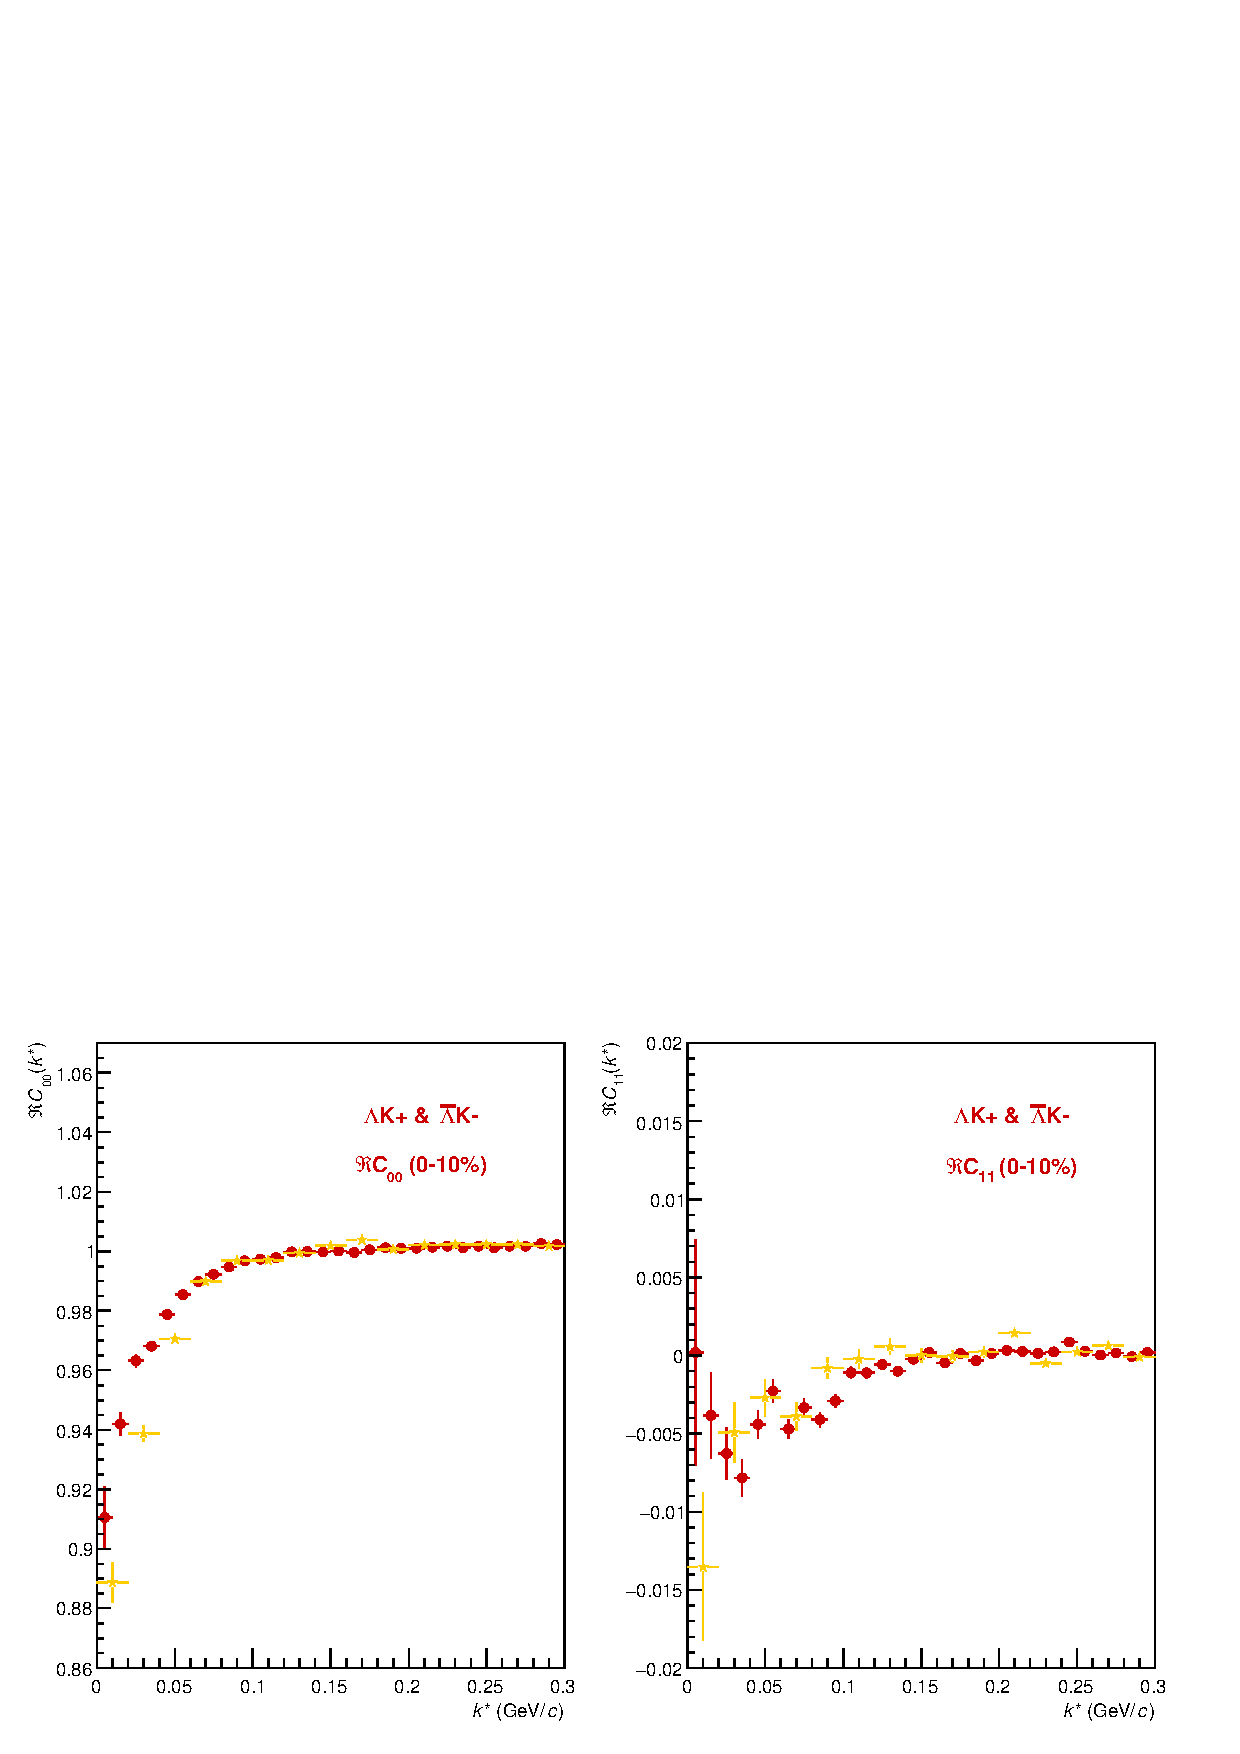
\includegraphics[width=0.8\textwidth]{\ResultsDirBase Results_cLamcKch_20181205/SphericalHarmonics/LamKchP/CanCfYlmReC00C11_LamKchPALamKchM_0010.pdf}
+  \includegraphics[width=0.8\textwidth]{\ResultsDirBase Results_cLamcKch_20181205/SphericalHarmonics/LamKchP/CanCfYlmReC00C11_LamKchPALamKchM_0010_wSysErr.pdf}
   \caption[\LamKchP $C_{00}$ and $\Re C_{11}$ Spherical Harmonic Components (0--10\%)]
   {
   (Color online) $C_{00}$ (left) and $\Re C_{11}$ (right) components of a spherical harmonic decomposition of the \LamKchP correlation function for the 0--10\% centrality bin.  
@@ -1090,7 +977,8 @@
   \label{fig:LamKchP_ReC00C11_0010}
 \end{figure}
 
-
+%************************************************************************************************************************
+%************************************************************************************************************************
 \section{Summary}
 \label{sec:Summary}
 
@@ -1131,82 +1019,15 @@
 %\input{}               %%%%%%%%%%% put your appendices here
 %
 
-%%%%%%%%%%%%%%%%%%%%%%%%%%%%%%%%%%%%%%%%%%%%%%%%%%%%%%%%%%%%%%%%%%%%%%%%%%%%%%%%%%%%%%%%%%%%%%%%%%%%%%%%%%%%%%%%%%%%%%%%%%
-\begin{comment}
-\begin{landscape}
-
-\section{$\lambda$ Parameters}
-\label{App:LamParams}
-
-\begin{table}[htbp]
- \centering
- \renewcommand{\arraystretch}{1.2}
- \resizebox{\paperwidth}{!}{
- \begin{tabular}{|c|cV{5.0}c|cV{5.0}c|cV{5.0}c|cV{5.0}c|cV{5.0}c|c|}
-  \multicolumn{2}{c}{\LamKchP} & \multicolumn{2}{c}{\ALamKchM} & \multicolumn{2}{c}{\LamKchM} & \multicolumn{2}{c}{\ALamKchP} & \multicolumn{2}{c}{\LamKs} & \multicolumn{2}{c}{\ALamKs} \\
-  \hline
-  \textbf{Pair System} & \textbf{$\lambda$ value} & \textbf{Pair System} & \textbf{$\lambda$ value} & \textbf{Pair System} & \textbf{$\lambda$ value} & \textbf{Pair System} & \textbf{$\lambda$ value} & \textbf{Pair System} & \textbf{$\lambda$ value} & \textbf{Pair System} & \textbf{$\lambda$ value} \\
-  \hlineB{3.0}
-  \multicolumn{12}{|c|}{3 Residuals (Max Parent $c\tau_{\mathrm{decay}}$ = 10 fm)} \\
-  \hlineB{3.0}
-  Primary & 0.527 & Primary & 0.526 & Primary & 0.526 & Primary & 0.527 & Primary & 0.543 & Primary & 0.544 \\
-  
-  $\Sigma^{0}$K$^{+}$ & 0.111 & $\overline{\Sigma}^{0}$K$^{-}$ & 0.110 & $\Sigma^{0}$K$^{-}$ & 0.110 & $\overline{\Sigma}^{0}$K$^{+}$ & 0.111 & $\Sigma^{0}$K$^{0}_{\mathrm{S}}$ & 0.120 & $\overline{\Sigma}^{0}$K$^{0}_{\mathrm{S}}$ & 0.120 \\
-  
-  $\Xi^{0}$K$^{+}$ & 0.039 & $\overline{\Xi}^{0}$K$^{-}$ & 0.035 & $\Xi^{0}$K$^{-}$ & 0.038 & $\overline{\Xi}^{0}$K$^{+}$ & 0.036 & $\Xi^{0}$K$^{0}_{\mathrm{S}}$ & 0.042 & $\overline{\Xi}^{0}$K$^{0}_{\mathrm{S}}$ & 0.039 \\
-  
-  $\Xi^{-}$K$^{+}$ & 0.050 & $\overline{\Xi}^{+}$K$^{-}$ & 0.046 & $\Xi^{-}$K$^{-}$ & 0.050 & $\overline{\Xi}^{+}$K$^{+}$ & 0.046 & $\Xi^{-}$K$^{0}_{\mathrm{S}}$ & 0.054 & $\overline{\Xi}^{+}$K$^{0}_{\mathrm{S}}$ & 0.050 \\
-  
-  Other & 0.226 & Other & 0.235 & Other & 0.228 & Other & 0.233 & Other & 0.194 & Other & 0.199 \\
-  
-  Fakes & 0.048 & Fakes & 0.048 & Fakes & 0.048 & Fakes & 0.048 & Fakes & 0.048 & Fakes & 0.048 \\
-  
-  \hlineB{3.0}  
-  \multicolumn{12}{|c|}{10 Residuals (Max Parent $c\tau_{\mathrm{decay}}$ = 4 fm)} \\
-  \hlineB{3.0}
-  Primary & 0.180 & Primary & 0.180 & Primary & 0.179 & Primary & 0.181 & Primary & 0.192 & Primary & 0.193 \\
-  
-  $\Sigma^{0}$K$^{+}$ & 0.116 & $\overline{\Sigma}^{0}$K$^{-}$ & 0.114 & $\Sigma^{0}$K$^{-}$ & 0.115 & $\overline{\Sigma}^{0}$K$^{+}$ & 0.116 & $\Sigma^{0}$K$^{0}_{\mathrm{S}}$ & 0.125 & $\overline{\Sigma}^{0}$K$^{0}_{\mathrm{S}}$ & 0.124 \\
-  
-  $\Xi^{0}$K$^{+}$ & 0.040 & $\overline{\Xi}^{0}$K$^{-}$ & 0.037 & $\Xi^{0}$K$^{-}$ & 0.040 & $\overline{\Xi}^{0}$K$^{+}$ & 0.037 & $\Xi^{0}$K$^{0}_{\mathrm{S}}$ & 0.043 & $\overline{\Xi}^{0}$K$^{0}_{\mathrm{S}}$ & 0.040 \\
-  
-  $\Xi^{-}$K$^{+}$ & 0.052 & $\overline{\Xi}^{+}$K$^{-}$ & 0.047 & $\Xi^{-}$K$^{-}$ & 0.052 & $\overline{\Xi}^{+}$K$^{+}$ & 0.048 & $\Xi^{-}$K$^{0}_{\mathrm{S}}$ & 0.056 & $\overline{\Xi}^{+}$K$^{0}_{\mathrm{S}}$ & 0.052 \\
-  
-  $\Sigma^{*+}$K$^{+}$ & 0.054 & $\overline{\Sigma}^{*-}$K$^{-}$ & 0.051 & $\Sigma^{*+}$K$^{-}$ & 0.053 & $\overline{\Sigma}^{*-}$K$^{+}$ & 0.051 & $\Sigma^{*+}$K$^{0}_{\mathrm{S}}$ & 0.058 & $\overline{\Sigma}^{*-}$K$^{0}_{\mathrm{S}}$ & 0.055 \\
-  
-  $\Sigma^{*-}$K$^{+}$ & 0.048 & $\overline{\Sigma}^{*+}$K$^{-}$ & 0.050 & $\Sigma^{*-}$K$^{-}$ & 0.048 & $\overline{\Sigma}^{*+}$K$^{+}$ & 0.050 & $\Sigma^{*-}$K$^{0}_{\mathrm{S}}$ & 0.052 & $\overline{\Sigma}^{*+}$K$^{0}_{\mathrm{S}}$ & 0.054 \\
-  
-  $\Sigma^{*0}$K$^{+}$ & 0.048 & $\overline{\Sigma}^{*0}$K$^{-}$ & 0.045 & $\Sigma^{*0}$K$^{-}$ & 0.048 & $\overline{\Sigma}^{*0}$K$^{+}$ & 0.045 & $\Sigma^{*0}$K$^{0}_{\mathrm{S}}$ & 0.052 & $\overline{\Sigma}^{*0}$K$^{0}_{\mathrm{S}}$ & 0.048 \\
-  
-  $\Lambda$K$^{*0}$ & 0.046 & $\overline{\Lambda}\overline{\mathrm{K}}^{*0}$ & 0.047 & $\Lambda\overline{\mathrm{K}}^{*0}$ & 0.046 & $\overline{\Lambda}$K$^{*0}$ & 0.047 & $\Lambda$K$^{*0}$ & 0.022 & $\overline{\Lambda}$K$^{*0}$ & 0.022 \\
-  
-  $\Sigma^{0}$K$^{*0}$ & 0.041 & $\overline{\Sigma}^{0}\overline{\mathrm{K}}^{*0}$ & 0.041 & $\Sigma^{0}\overline{\mathrm{K}}^{*0}$ & 0.041 & $\overline{\Sigma}^{0}$K$^{*0}$ & 0.041 & $\Sigma^{0}$K$^{*0}$ & 0.019 & $\overline{\Sigma}^{0}$K$^{*0}$ & 0.019 \\
-  
-  $\Xi^{0}$K$^{*0}$ & 0.014 & $\overline{\Xi}^{0}\overline{\mathrm{K}}^{*0}$ & 0.013 & $\Xi^{0}\overline{\mathrm{K}}^{*0}$ & 0.014 & $\overline{\Xi}^{0}$K$^{*0}$ & 0.013 & $\Xi^{0}$K$^{*0}$ & 0.007 & $\overline{\Xi}^{0}$K$^{*0}$ & 0.006 \\
-  
-  $\Xi^{-}$K$^{*0}$ & 0.018 & $\overline{\Xi}^{+}\overline{\mathrm{K}}^{*0}$ & 0.017 & $\Xi^{-}\overline{\mathrm{K}}^{*0}$ & 0.018 & $\overline{\Xi}^{+}$K$^{*0}$ & 0.017 & $\Xi^{-}$K$^{*0}$ & 0.009 & $\overline{\Xi}^{+}$K$^{*0}$ & 0.008 \\
-  
-  Other & 0.295 & Other & 0.310 & Other & 0.299 & Other & 0.307 & Other & 0.318 & Other & 0.330 \\
-  
-  Fakes & 0.048 & Fakes & 0.048 & Fakes & 0.048 & Fakes & 0.048 & Fakes & 0.048 & Fakes & 0.048 \\
-  
-  \hlineB{3.0}
- \end{tabular}}
- \caption{$\lambda$ values for the individual components of the \LamK correlation functions for the case of 3 and 10 residual contributions.}
- \label{tab:LambdaValues_All}
-\end{table}
-
-\end{landscape}
-\end{comment}
-%%%%%%%%%%%%%%%%%%%%%%%%%%%%%%%%%%%%%%%%%%%%%%%%%%%%%%%%%%%%%%%%%%%%%%%%%%%%%%%%%%%%%%%%%%%%%%%%%%%%%%%%%%%%%%%%%%%%%%%%%%
-
-
+%************************************************************************************************************************
+%************************************************************************************************************************
 \section{Stavinskiy Reference Method}
 \label{App:StavMethod}
 
 Another option for obtaining the reference distribution, $B(k^{*})$, is to use, what will be referred to as, the ``Stavinskiy method" \cite{Stavinskiy04}.
 The method was first proposed to handle the case of one event femtoscopy, and has been suggested for use in eliminating momentum conservation effects in the reference distribution \cite{Lisa:2005dd}.
 The method is appropriate for collisions between symmetric projectiles, at sufficiently large energy, with a detector which is symmetrical with respect to the transition $\mathbf{r} \rightarrow \mathbf{-r}$.
+The use of this method in a three-dimensional analysis of two-pion correlations produced, in comparison to the event mixing results, an increase of 6\% for $R_{\mathrm{side}}$ at low-$k_{\mathrm{T}}$ and up to 4\% for $R_{\mathrm{out}}$ and $R_{\mathrm{long}}$ \cite{Aamodt:2011mr}.
 The purpose of using the Stavinskiy method in this \LamK analysis is to rid the correlation functions of the non-femtoscopic background.  
 More specifically, the intent is to handle background contributions from elliptic flow, and other sources having reflection symmetry in the transverse plane.  
 With the Stavinskiy method, mixed-event pairs are not used for the reference distribution; instead, same-event pseudo-pairs, formed by rotating one particle in a real pair by 180$^\circ$ in the transverse plane, are used.  
@@ -1215,24 +1036,9 @@
 The results of correctly implementing such a procedure are shown in Figure \ref{fig:StavCfs_Correct_LamKchP}.  
 The figure shows the Stavinskiy method does a very good job of ridding the \LamKchP correlations of their non-femtoscopic backgrounds.  
 
-%%%%%%%%%%%%%%%%%%%%%%%%%%%%%%%%%%%%%%%%%%%%%%%%%%%%%%%%%%%%%%%%%%%%%%%%%%%%%%%%%%%%%%%%%%%%%%%%%%%%%%%%%%%%%
-\begin{comment}
 \begin{figure}[h!]
   \centering
-  \includegraphics[width=\textwidth]{/home/jesse/Analysis/FemtoAnalysis/AnalysisNotes/4_CorrelationFunctions/Figures/OnlyTwo/canKStarCfsLamKchPwConj_20180505vs20180505StavCf_CustomRebin.pdf}
-  \caption[\LamKchP Stavinskiy Correlation Functions]
-  {
-  \LamKchPALamKchM correlation functions built using the Stavinskiy method for 0--10\%, 10--30\%, and 30--50\% centralities.  
-  Closed (red) symbols represent correlations built using the normal mixed-event reference distribution, while open (green) symbols represent correlations formed using the Stavinskiy same-event pseudo-pairs as a reference.
-  }
-  \label{fig:StavCfs_Correct_LamKchP}
-\end{figure}
-\end{comment}
-%%%%%%%%%%%%%%%%%%%%%%%%%%%%%%%%%%%%%%%%%%%%%%%%%%%%%%%%%%%%%%%%%%%%%%%%%%%%%%%%%%%%%%%%%%%%%%%%%%%%%%%%%%%%%
-
-\begin{figure}[h!]
-  \centering
-  \includegraphics[width=0.667\textwidth]{/home/jesse/Analysis/FemtoAnalysis/AnalysisNotes/4_CorrelationFunctions/Figures/OnlyTwo/canKStarCfsLamKchPCombConj_20180505vs20180505StavCf_CustomRebin.pdf}
+  \includegraphics[width=0.667\textwidth]{/home/jesse/Analysis/FemtoAnalysis/AnalysisNotes/4_CorrelationFunctions/Figures/OnlyTwo/canKStarCfsLamKchPCombConj_20190319vs20190319StavCf_CustomRebin.pdf}
   \caption[\LamKchP Stavinskiy Correlation Functions]
   {
   (Color online) \LamKchPALamKchM correlation functions built using the Stavinskiy method for 0--10\%, 10--30\%, and 30--50\% centralities.  Closed symbols represent correlations built using the normal mixed-event reference distribution, while open symbols represent correlations formed using the Stavinskiy same-event pseudo-pairs as a reference.
@@ -1242,8 +1048,8 @@
 
 
 
-%%%%%%%%%%%%%%%%%%%%%%%%%%%%%%%%%%%%%%%%%%%%%%%%%%%%%%%%%%%%%%%%%%%%%%%%%%%%%%%%%%%%%%%%%%%%%%%%%%%%%%%%%%%%%
-\begin{comment}
+%************************************************************************************************************************
+%************************************************************************************************************************
 \section{Strong and Coulomb Fitter}
 \label{App:CoulombFitter}
 
@@ -1275,94 +1081,94 @@
 To build a fit function for a system including both strong and Coulomb interactions two related options were considered. 
 The first option was to numerically integrate Eq.\ \ref{eqn:KooninPrattEqn}.  
 The second option was to simulate a large sample of particle pairs, calculate the wave function describing the interaction, and average to obtain the integral in Eq.\ \ref{eqn:KooninPrattEqn}. 
-\end{comment}
-%%%%%%%%%%%%%%%%%%%%%%%%%%%%%%%%%%%%%%%%%%%%%%%%%%%%%%%%%%%%%%%%%%%%%%%%%%%%%%%%%%%%%%%%%%%%%%%%%%%%%%%%%%%%%
-
-
-%%%%%%%%%%%%%%%%%%%%%%%%%%%%%%%%%%%%%%%%%%%%%%%%%%%%%%%%%%%%%%%%%%%%%%%%%%%%%%%%%%%%%%%%%%%%%%%%%%%%%%%%%%%%%%%%%%%%%%%%%
-\begin{comment}
-\section{Spherical Harmonic Decomposition}
-\label{app:SphericalHarmonics}
-
-
-In Fig.\ \ref{fig:LamKchP_ReC00C11_0010} results are shown for the $C_{00}$ and $\Re C_{11}$ components from the spherical decomposition of our \LamKchP system in the 0--10\% centrality bin.
-As seen in the figure, the $C_{00}$ signal is similar to that observed in the one-dimensional study.
-The $\Re C_{11}$ component shows a clear deviation from zero, and the negative value signifies that the \Lam particles are, on average, emitted further out and/or earlier than the K mesons.
+
+
+%************************************************************************************************************************
+%************************************************************************************************************************
+\section{Relative Emission Shifts with THERMINATOR 2}
+\label{App:THERM}
+
+Fig.\ \ref{fig:LamKchP_StdThermSources} shows \LamKchP results from the THERMINATOR 2 event generator for an impact parameter of $b = 2$ fm.
+As THERMINATOR 2 does not include any final state effects, the femtoscopic correlation was introduced by assuming a set of scattering parameters ($\Re f_{0},\, \Im f_{0},\, d_{0}$) = ($-$0.60 fm, 0.51 fm, 0.83 fm) and weighting the signal distribution (numerator pairs) with the modulus squared of the two-particle wave function, $|\Psi|^{2}$.
+
+The top row of Fig. \ref{fig:LamKchP_StdThermSources} shows the experimental $\Lambda\mathrm{K}^{+}\oplus\overline{\Lambda}\mathrm{K}^{-}$ data together with the simulation results for the one-dimension correlation function (top left) and for the $\Re C_{11}$ component of the spherical harmonic decomposition (top right).
+The other four plots in Fig.\ \ref{fig:LamKchP_StdThermSources} show the source distribution from the simulation in the out (middle left), side (middle right), and long (bottom left) directions, as well as the temporal characteristics of the source (bottom right), all measured in the PRF.
+The source distributions have all been fitted with a Gaussian form, the results of which are printed within the respective plots.
+One immediately sees a significant spatial shift in the out direction, $\mu_{\mathrm{out}} \approx$ 4 fm, and negligible shift in the other two directions, $\mu_{\mathrm{side}} \approx \mu_{\mathrm{long}} \approx$ 0 fm.
+In other words, the figure demonstrates that, within the THERMINATOR 2 model, the \Lam is, on average, emitted further out than its K partner.
+Additionally, the figure shows a nonzero temporal shift, $\mu_{\Delta t} \approx$ $-$2.7 fm/$c$, signifying that the \Lam is, on average, emitted earlier than its K partner within the model. 
 
 
 \begin{figure}[h!]
   \centering
-  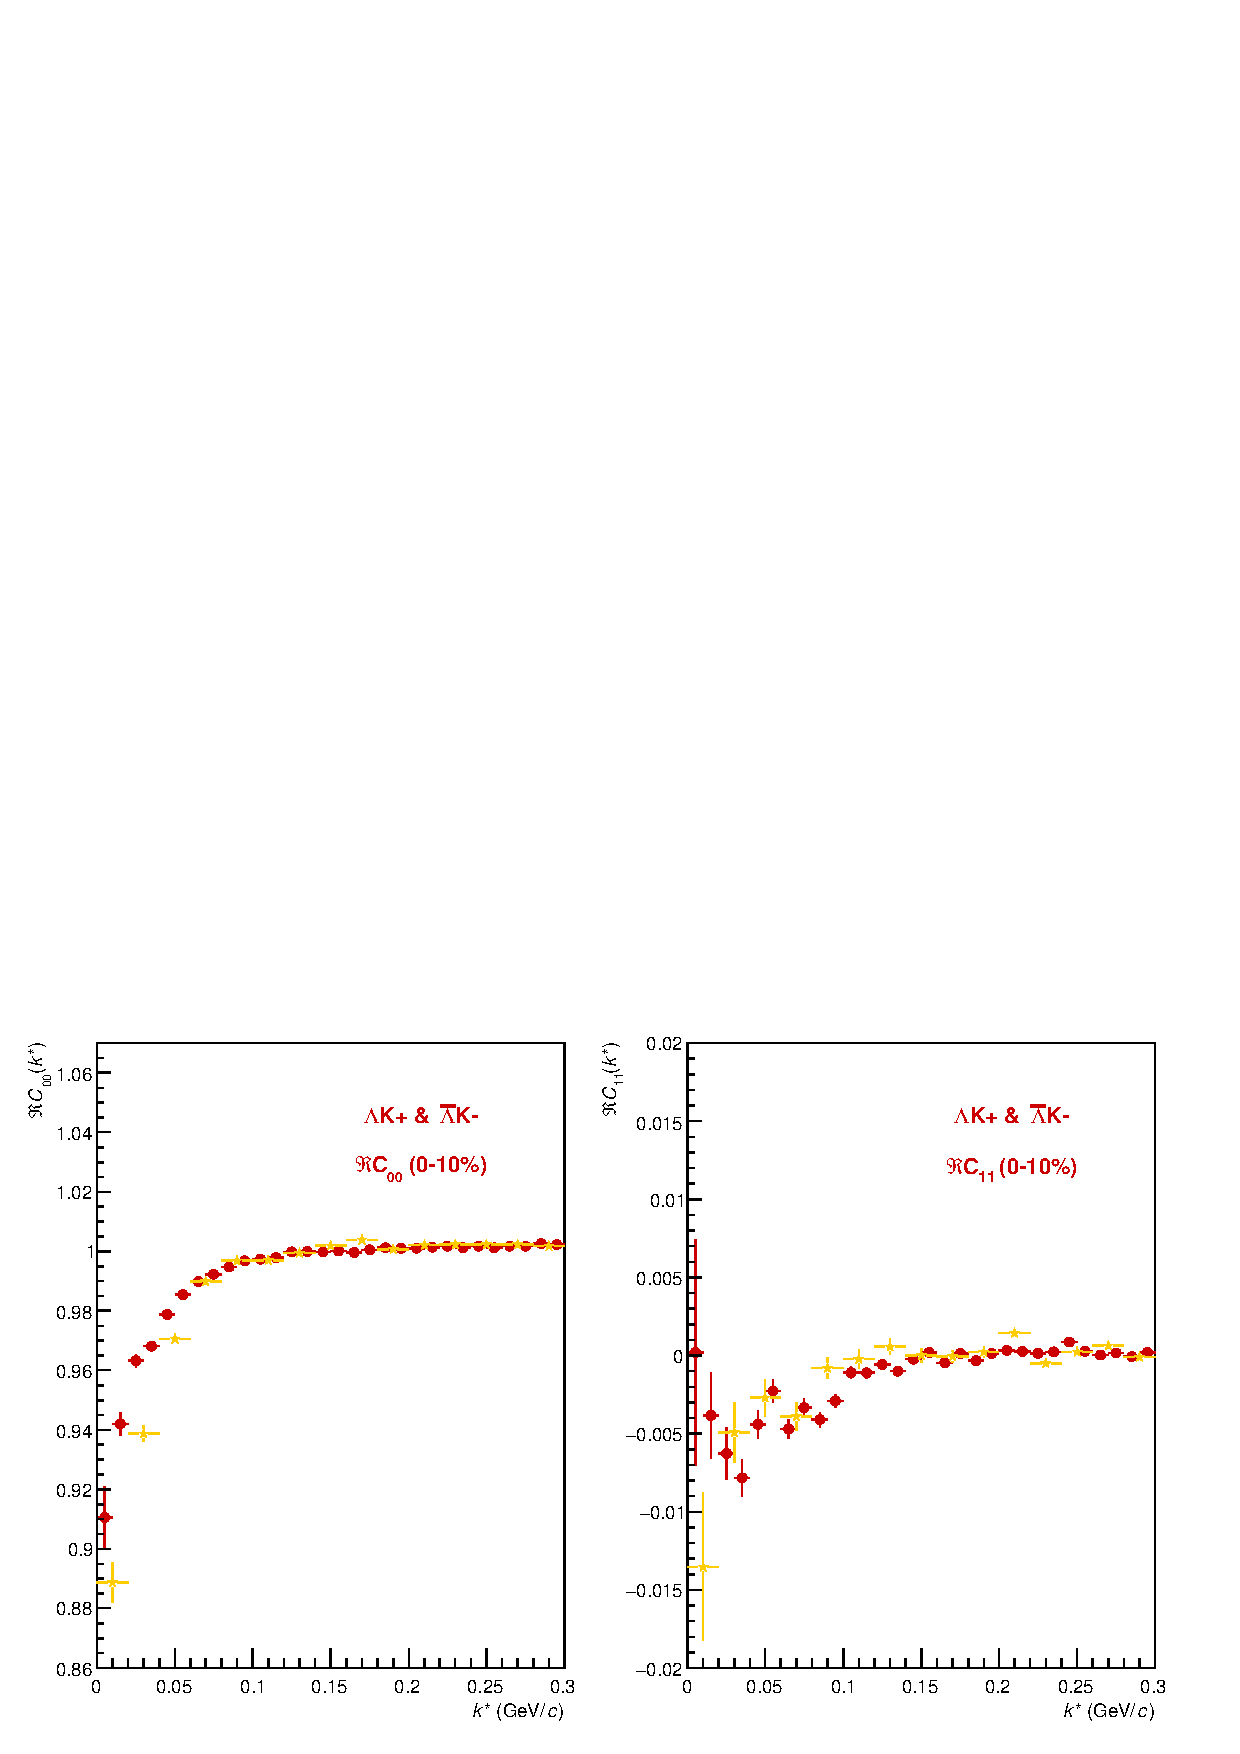
\includegraphics[width=0.8\textwidth]{\ResultsDirBase Results_cLamcKch_20181205/SphericalHarmonics/LamKchP/CanCfYlmReC00C11_LamKchPALamKchM_0010.pdf}
-  \caption[\LamKchP $C_{00}$ and $\Re C_{11}$ Spherical Harmonic Components (0--10\%)]{$C_{00}$ (left) and $\Re C_{11}$ (right) components of a spherical harmonic decomposition of the \LamKchP correlation function for the 0--10\% centrality bin.  
-The $C_{00}$ component is similar to the 1D correlation functions typically studied, and probes the overall size of the source.
-The $\Re C_{11}$ component probes the asymmetry in the system; a non-zero value reveals the asymmetry}
-  \label{fig:LamKchP_ReC00C11_0010}
+  \includegraphics[width=0.8\textwidth]{/home/jesse/Analysis/FemtoAnalysis/AnalysisNotes/7_ResultsAndDiscussion/7.1_ResultsLamK/7.1.2_ResultsLamK_DiscussionOfmTScaling/ThermPlots/LamKchP/CanCfwSourceAndDeltaTwC11wData_Full_LamKchP_3dHistPairSource3d_oslLamKchP_FromFileCorrelationFunctions_BuildCfYlm.pdf}
+  \caption[THERMINATOR 2 simulatin for \LamKchP]
+  {
+  Results from the THERMINATOR 2 simulation implemented with an impact parameter $b = 2$ fm for the \LamKchP pair system.
+  (Top left) the one-dimensional correlation function from THERMINATOR 2 together with the experimental data.
+  (Top right) the $\Re C_{11}$ component of a spherical harmonic decomposition of the THERMINATOR 2 simulation together with the experimental data.
+  The other four panels show the source distribution from the simulation in the out (middle left), side (middle right), and long (bottom left) directions, as well as the temporal characteristics (bottom right), all in the PRF.
+  The source distributions have all been fitted with a Gaussian form, the results of which are printed within the respective plots.
+  }
+  \label{fig:LamKchP_StdThermSources}
 \end{figure}
-\end{comment}
-%%%%%%%%%%%%%%%%%%%%%%%%%%%%%%%%%%%%%%%%%%%%%%%%%%%%%%%%%%%%%%%%%%%%%%%%%%%%%%%%%%%%%%%%%%%%%%%%%%%%%%%%%%%%%%%%%%%%%%%%%
-
-\section{Relative Emission Shifts with THERMINATOR 2}
-\label{App:THERM}
-
-Fig.\ \ref{fig:LamKchP_StdThermSources} shows results from the THERMINATOR 2 event generator for an impact parameter of $b = 2$ fm.
-As THERMINATOR 2 does not include any final state effects, the femtoscopic correlation was introduced by assuming a set of scattering parameters ($\Re f_{0}, \Im f_{0}, d_{0}$) = ($-1.16, 0.51, 1.08$) and weighting the signal distribution (numerator pairs) with the modulus squared of the two-particle wave function, $|\Psi|^{2}$.
-
-The top left of Fig.\ \ref{fig:LamKchP_StdThermSources_Spatial} shows a fit to the one-dimensional correlation function from THERMINATOR 2.
-The scattering parameters are known precisely here, as they served as the weights used in the simulation, and are kept constant in the fit.
-Only the extracted one-dimensional source size is of interest here, so the $\lambda$ parameter is also fixed at unity.
-The other three plots in Fig.\ \ref{fig:LamKchP_StdThermSources_Spatial} show the source distribution in the out (top right), side (bottom left), and long (bottom right) directions (all in the PRF).
-The source distributions have all been fitted with a Gaussian form, the result of which is printed within the respective plot.
-One immediately sees a significant shift in the out direction, $\mu_{\mathrm{out}} \approx$ 4 fm, and negligible shift in the other two directions, $\mu_{\mathrm{side}} \approx \mu_{\mathrm{long}} \approx$ 0 fm.
-The figure demonstrates that, within the THERMINATOR 2 model, the \Lam is, on average, emitted further out that its K partner.
-Finally, Fig.\ \ref{fig:LamKchP_StdThermSources_Temporal} shows the distribution of the relative time of emittance, again in the PRF.
-The figure shows that the \Lam is, on average, emitted earlier than its K partner. 
+
+
 
 This section concludes with a brief look at how a spatial separation of the single particle sources affects the radii extracted from a femtoscopic analysis.
 To achieve this, THERMINATOR 2 is used in a similar fashion as described above, but with one important difference.
 Instead of taking the source information from THERMINATOR 2, the source is drawn from a pre-determined Gaussian distribution.
-In all cases, $R_{\mathrm{out}} = R_{\mathrm{side}} = R_{\mathrm{long}}$ = 5 fm, and $\mu_{\mathrm{side}} = \mu_{\mathrm{long}}$ = 0 fm.
-In Figure \ref{fig:LamKchP_ThermSources_VaryMuOut}, results are shown for the case of $\mu_{\mathrm{out}}$ = 1 fm, $\mu_{\mathrm{out}}$ = 3 fm, and $\mu_{\mathrm{out}}$ = 6 fm.
-In this figure, the side and long distributions are not shown, as they are simple Gaussians of width 5 fm centered about the origin.
+In all, $R_{\mathrm{out}} = R_{\mathrm{side}} = R_{\mathrm{long}}$ = 5 fm, and $\mu_{\mathrm{side}} = \mu_{\mathrm{long}}$ = 0 fm.
+The cases of $\mu_{\mathrm{out}}$ = 0 fm, $\mu_{\mathrm{out}}$ = 1 fm, $\mu_{\mathrm{out}}$ = 3 fm, and $\mu_{\mathrm{out}}$ = 6 fm were studied within the simulation.
+Note, within this implementation there is no time difference in the emission of the \Lam and K particles.
+For each, a one-dimensional correlation function is generated and fit with the Lednick\'y model, as shown in Fig.\ \ref{fig:LamKchP_ThermSources_VaryMuOut}).
+The scattering parameters are known precisely here, as they served as the weights used in the simulation, and are kept constant in the fit.
+Only the extracted one-dimensional source size is of interest here, so the $\lambda$ parameter is also fixed at unity.
 The figure demonstrates that as the separation $\mu_{\mathrm{out}}$ increases, so do the extracted femtoscopic radii.
-
-\begin{figure}[h!]
-  \centering
-  %%----start of first subfigure---  
-  \subfigure[(Top Left) Simple fit on simulation from THERMINATOR 2. Generated source in the (Top Right) out, (Bottom Left) side, and (Bottom Right) long directions.]{
-    \label{fig:LamKchP_StdThermSources_Spatial}
-    \includegraphics[width=\linewidth]{/home/jesse/Analysis/FemtoAnalysis/AnalysisNotes/7_ResultsAndDiscussion/7.1_ResultsLamK/7.1.2_ResultsLamK_DiscussionOfmTScaling/ThermPlots/LamKchP/CanCfwSource_Full_LamKchP_3dHistPairSource3d_oslLamKchP_FromFileCorrelationFunctions_wOtherPairs.pdf}} \\
-  %%----start of second subfigure---
-  \subfigure[Temporal characteristics of the source.]{
-    \label{fig:LamKchP_StdThermSources_Temporal}
-    \includegraphics[width=0.60\linewidth]{/home/jesse/Analysis/FemtoAnalysis/AnalysisNotes/7_ResultsAndDiscussion/7.1_ResultsLamK/7.1.2_ResultsLamK_DiscussionOfmTScaling/ThermPlots/LamKchP/CanDeltaT_Full_LamKchP_FromFileCorrelationFunctions_wOtherPairs_BuildCfYlm.pdf}}  
-  %%----overall caption----
-  \caption[Extracted Radius and Pair Sources from THERMINATOR 2]
-  {
-  (Color online) Extracted radius when performing a simple fit on simulation from THERMINATOR 2, along with the spatio-temporal characteristics generated by the simulation.
-  }
-  \label{fig:LamKchP_StdThermSources}
-\end{figure}
+Figure \ref{fig:LamKchP_ThermSources_VaryMuOut_SH} shows, together with the experimental \LamKchP data, the effect of increasing $\mu_{\mathrm{out}}$ on the $\Re C_{00}$ and $\Re C_{11}$ components of the spherical harmonic decomposition.
+The figures shows that as $\mu_{\mathrm{out}}$ increases, so does the magnitude of the $\Re C_{11}$ signal.
+
+
 
 
 
 \begin{figure}[h]
   \centering
-  \includegraphics[width=\textwidth]{/home/jesse/Analysis/FemtoAnalysis/AnalysisNotes/7_ResultsAndDiscussion/7.1_ResultsLamK/7.1.2_ResultsLamK_DiscussionOfmTScaling/ThermPlots/LamKchP/CanCompMus_Full_LamKchP_3dHistPairSource3d_oslLamKchP.pdf}
+  \includegraphics[width=\textwidth]{/home/jesse/Analysis/FemtoAnalysis/AnalysisNotes/7_ResultsAndDiscussion/7.1_ResultsLamK/7.1.2_ResultsLamK_DiscussionOfmTScaling/ThermPlots/LamKchP/CanPartCompMus_Full_LamKchP_3dHistPairSource3d_oslLamKchP.pdf}
   \caption[Varying $\mu_{\mathrm{Out}}$ with THERMINATOR 2]
   {
-  (Color online) Probing the effect of varying the source shift in the outward direction, $\mu_{\mathrm{out}}$, within the THERMINATOR 2 framework.  
+  Probing the effect of varying the source shift in the outward direction, $\mu_{\mathrm{out}}$, within the THERMINATOR 2 framework.  
   To achieve this, particle pairs are formed from the simulation, but with altered spatial characteristics achieved by drawing the out, side, and long components from predetermined Gaussian distributions.  
-  The plots on the left show fits resulting from the sources (in the out direction) shown on the right.  
-  The sources in the side and long directions are not shown, and are both Gaussians of width 5 fm centered at the origin for all cases.  
-  Moving from top to bottom, $\mu_{\mathrm{out}}$ increase from 0 to 6 fm, the effect of which clearly increases the effective radius extracted in the fit.
+  The sources in all three directions are Gaussians of width 5 fm.
+  The distributions used for the side and long direction are centered at the origin, while the shift in the outward direction, $\mu_{\mathrm{out}}$, is varied.
+  The plots show fits resulting from sources with $\mu_{\mathrm{out}}$ increasing from 0 to 6 fm. 
+  The effect of increasing $\mu_{\mathrm{out}}$ clearly increases the effective radius extracted in the fit.
   }
   \label{fig:LamKchP_ThermSources_VaryMuOut}
 \end{figure}
 
+
+
+\begin{figure}[h]
+  \centering
+  \includegraphics[width=\textwidth]{/home/jesse/Analysis/FemtoAnalysis/AnalysisNotes/7_ResultsAndDiscussion/7.1_ResultsLamK/7.1.2_ResultsLamK_DiscussionOfmTScaling/ThermPlots/LamKchP/CanCompFourThermCfYlmReC00C11_Full_RandomEPs_LamKchPALamKchM.pdf}
+  \caption[\LamKchP $C_{00}$ and $\Re C_{11}$ Spherical Harmonic Components (0--10\%) with THERMINATOR 2 ($b = 2$ fm]
+  {
+  (Color online) $C_{00}$ (left) and $\Re C_{11}$ (right) components of a spherical harmonic decomposition of the \LamKchP correlation function for the 0--10\% centrality bin shown with results from the THERMINATOR 2 simulation implemented with different shifts in the outward direction, $\mu_{\mathrm{out}}$, as described in the text.
+  }
+  \label{fig:LamKchP_ThermSources_VaryMuOut_SH}
+\end{figure}
+
+
+
+
+
+
 \clearpage
 
 
-
+%************************************************************************************************************************
+%************************************************************************************************************************
 \section{The ALICE Collaboration}
 \label{app:collab}
 %\input{authorlist-preprint.tex}  %%%%%%% done by webmaster team
